\documentclass{beamer}
\usepackage{tcolorbox}
\usepackage{caption}
\usepackage{tikz}
\usepackage{pgfplots}
\usepackage{adjustbox}
\usepackage{pgfplots}
\usepackage{multicol}
\usepackage{pdfpages}
%\beamerdefaultoverlayspecification{<+->}
\newcommand{\data}{\mathcal{D}}

\setlength{\abovedisplayskip}{1pt}
\setlength{\belowdisplayskip}{1pt}

\makeatletter
\def\magicomadjust{0em}  % a way to adjust if the spacing should be different
\newdimen\indent@amount
\def\magicom{\relax
  \ifhmode $$%
    \predisplaypenalty\@M \postdisplaypenalty\@M
    \abovedisplayskip-\baselineskip \belowdisplayskip\z@
    \abovedisplayshortskip\abovedisplayskip
    \belowdisplayshortskip\belowdisplayskip
    \global\indent@amount\predisplaysize
     $$\count@\prevgraf \advance\count@-\thr@@
         \prevgraf\count@
    \global\advance\indent@amount-2em  % correction for \predisplaysize indent
    \global\advance\indent@amount\magicomadjust  % correction for verse env, for example
    \hspace*\indent@amount
  \else\typeout{*Not in hmode*}\fi}
\makeatother



\DeclareMathOperator*{\argmin}{arg\,min}

\newcommand\Item[1][]{%
	\ifx\relax#1\relax  \item \else \item[#1] \fi
	\abovedisplayskip=0pt\abovedisplayshortskip=0pt~\vspace*{-\baselineskip}}


\usetheme{metropolis}           % Use metropolis theme


\title{Support Vector Machines}
\date{\today}
\author{Nipun Batra}
\institute{IIT Gandhinagar}

\begin{document}
\maketitle


{
	\setbeamercolor{background canvas}{bg=}
	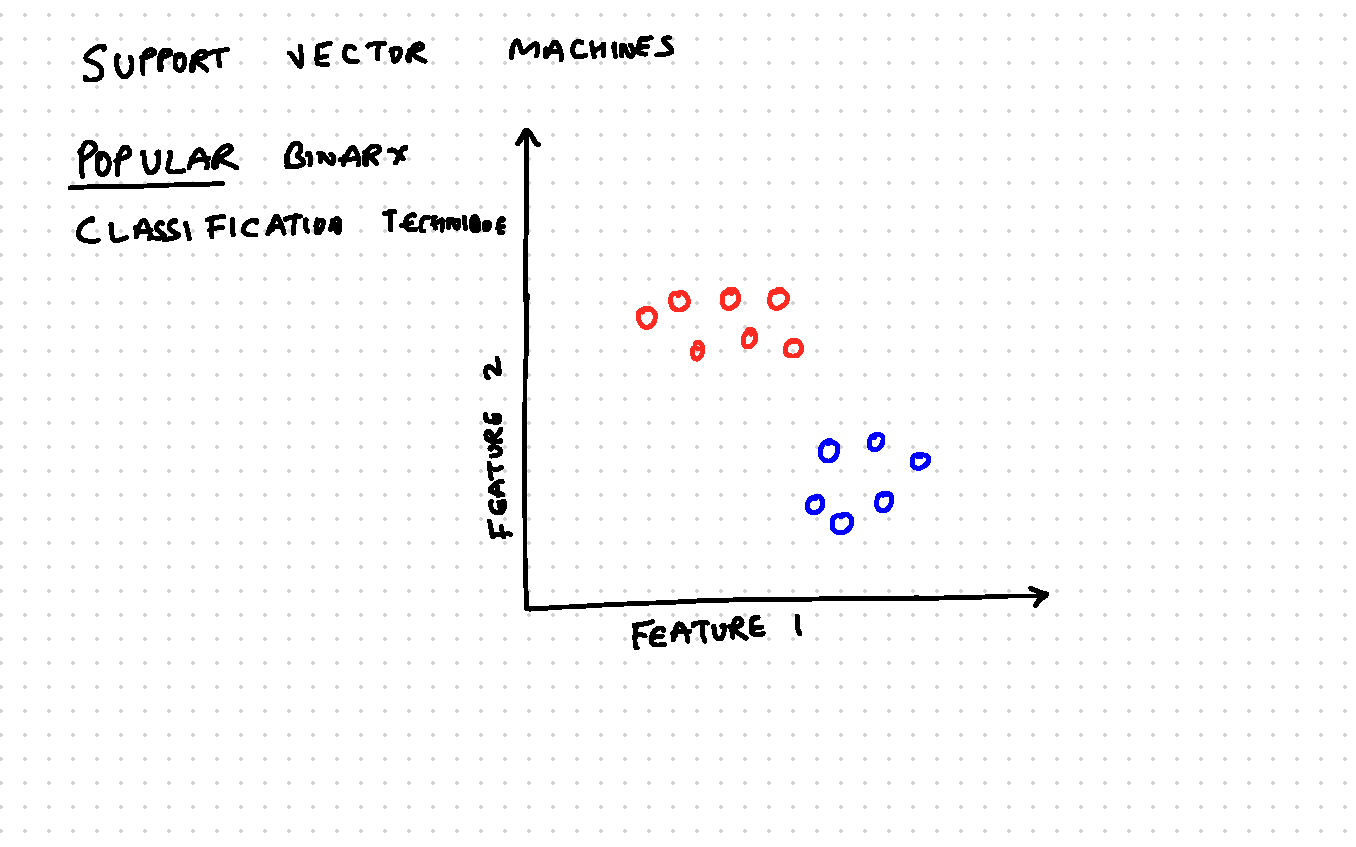
\includepdf[page=1-19]{svm/Svm-notes.pdf}
}





\begin{frame}{Distance between 2 parallel hyperplanes}
Equation of two planes is:
$$
\begin{aligned}
&\vec{w}\cdot \vec{x}+b_1=0\\
&\vec{w}\cdot \vec{x}+b_2=0
\end{aligned}
$$

\pause For a point $\vec{x_1}$ on plane 1 and $\vec{x_2}$ on plane 2, we have:
\pause $$
\begin{array}{l}
{\overrightarrow{x_{2}}=\overrightarrow{x_{1}}+t \vec{w}} \\
{D=|t \vec{w}|=|t|||\vec{w}| |}
\end{array}
$$

\pause We can rewrite as follows:
\pause $$
\begin{array}{c}
{\vec{w} \cdot \vec{x}_{2}+b_{2}=0} \\
{\Rightarrow \vec{w} \cdot\left(\vec{x}_{1}+t \vec{w}\right)+b_{2}=0}
\end{array}
$$
\pause $$
\Rightarrow \vec{w} \cdot \vec{x}_{1}+t\|\vec{w}\|^{2}+b_1-b_1+b_2 = 0
\Rightarrow t = \frac{b_1 - b_2}{\|\vec{w}\|^{2}}  \Rightarrow D = t\|\vec{w}\| =  \frac{b_1 - b_2}{\|\vec{w}\|}
$$
\end{frame}

{
	\setbeamercolor{background canvas}{bg=}
	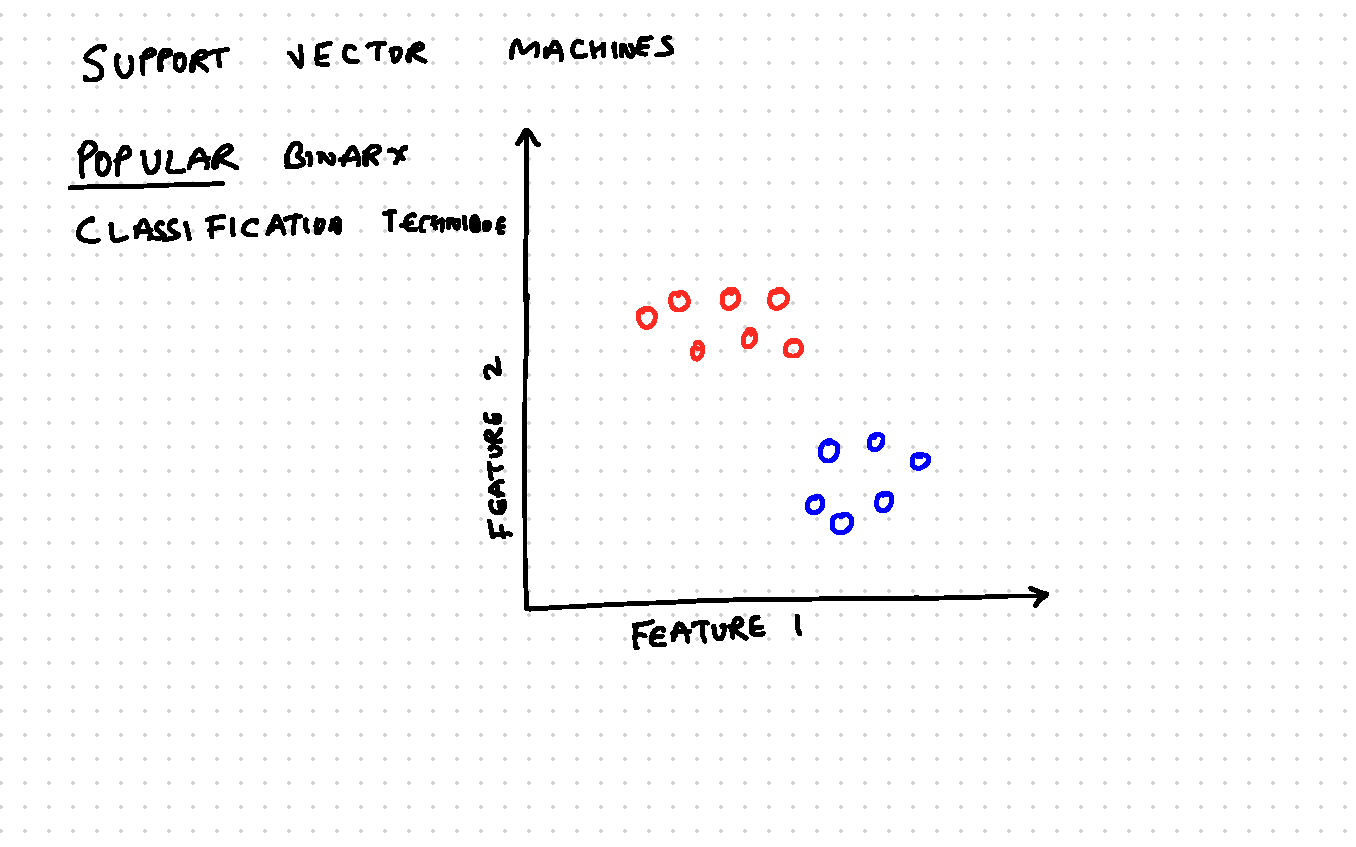
\includepdf[page=20-25]{svm/Svm-notes.pdf}
}





\begin{frame}{Primal Formulation}
	\begin{tcolorbox}{Objective}
	\begin{align*}
	\text{Minimize } & \frac{1}{2}||w||^{2} \\
	\text{s.t. } & y_{i}(w.x_{i} + b) \geq 1 \hspace{2mm}\forall i
	\end{align*}
\end{tcolorbox}
\pause 
Q) What is $||w||$?
\pause
\begin{multicols}{2}
\begin{equation*}
	 w = \begin{bmatrix}
	 w_{1} \\
     w_{2} \\
     ...  \\
     w_{n} \\
	\end{bmatrix}
\end{equation*}\break
\begin{align*}
	 ||w|| &= \sqrt{w^{T}w}\\
	 &= \sqrt{\begin{bmatrix}
	 w_{1}, w_{2}, ... w_{n}
	 \end{bmatrix}
	 \begin{bmatrix}
	  w_{1} \\
	  w_{2} \\
     ...  \\
     w_{n} \\
	 \end{bmatrix}}
\end{align*}

\end{multicols}

\end{frame}

{
	\setbeamercolor{background canvas}{bg=}
	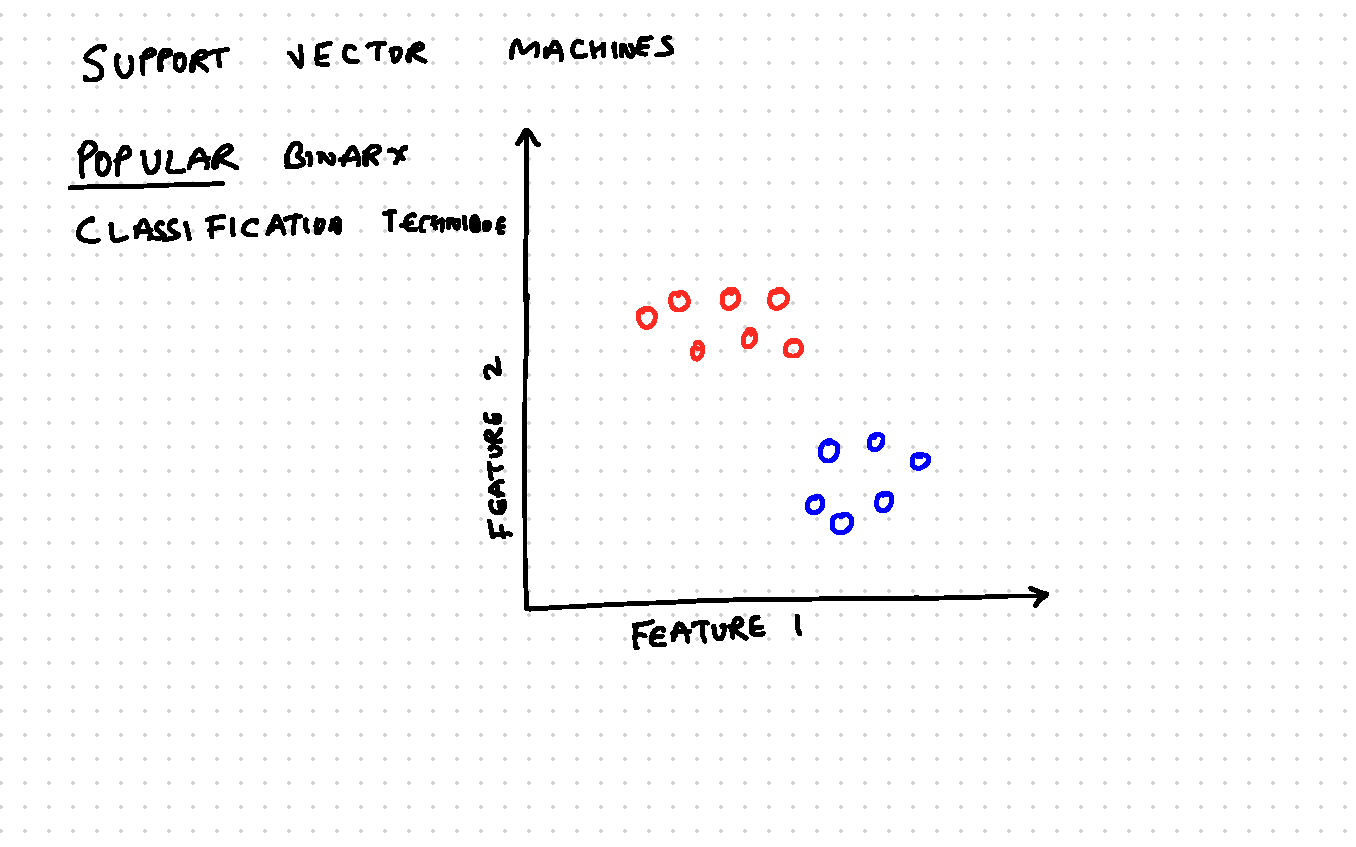
\includepdf[page=27]{svm/Svm-notes.pdf}
}



\begin{frame}{Simple Exercise}

\begin{align*}
\begin{bmatrix}
x && y \\
1 && 1\\
2 && 1\\
-1 && -1\\
-2 && -1\\
\end{bmatrix}
\end{align*}
Separating Hyperplane: $wx + b = 0$
\end{frame}

\begin{frame}{Simple Exercise}
\begin{tcolorbox}

\begin{equation*}
y_{i}(w_{i}x_{i} + b) \geq 1
\end{equation*}
\end{tcolorbox}
\begin{multicols}{2}
\begin{equation*}
\begin{bmatrix}
x_{1} && y \\
1 && 1\\
2 && 1\\
-1 && -1\\
-2 && -1\\
\end{bmatrix}
\end{equation*}\break

\begin{align*}
&\Rightarrow y_{i}(w_{i}x_{i} + b) \geq 1\\
&\Rightarrow 1(w_{1} + b) \geq 1\\
&\Rightarrow 1(2w_{1} + b)\geq 1\\
&\Rightarrow -1(-w_{1}+b) \geq 1\\
&\Rightarrow -1(-2w_{1}+b) \geq 1\\
\end{align*}


\end{multicols}
\end{frame}

{
	\setbeamercolor{background canvas}{bg=}
	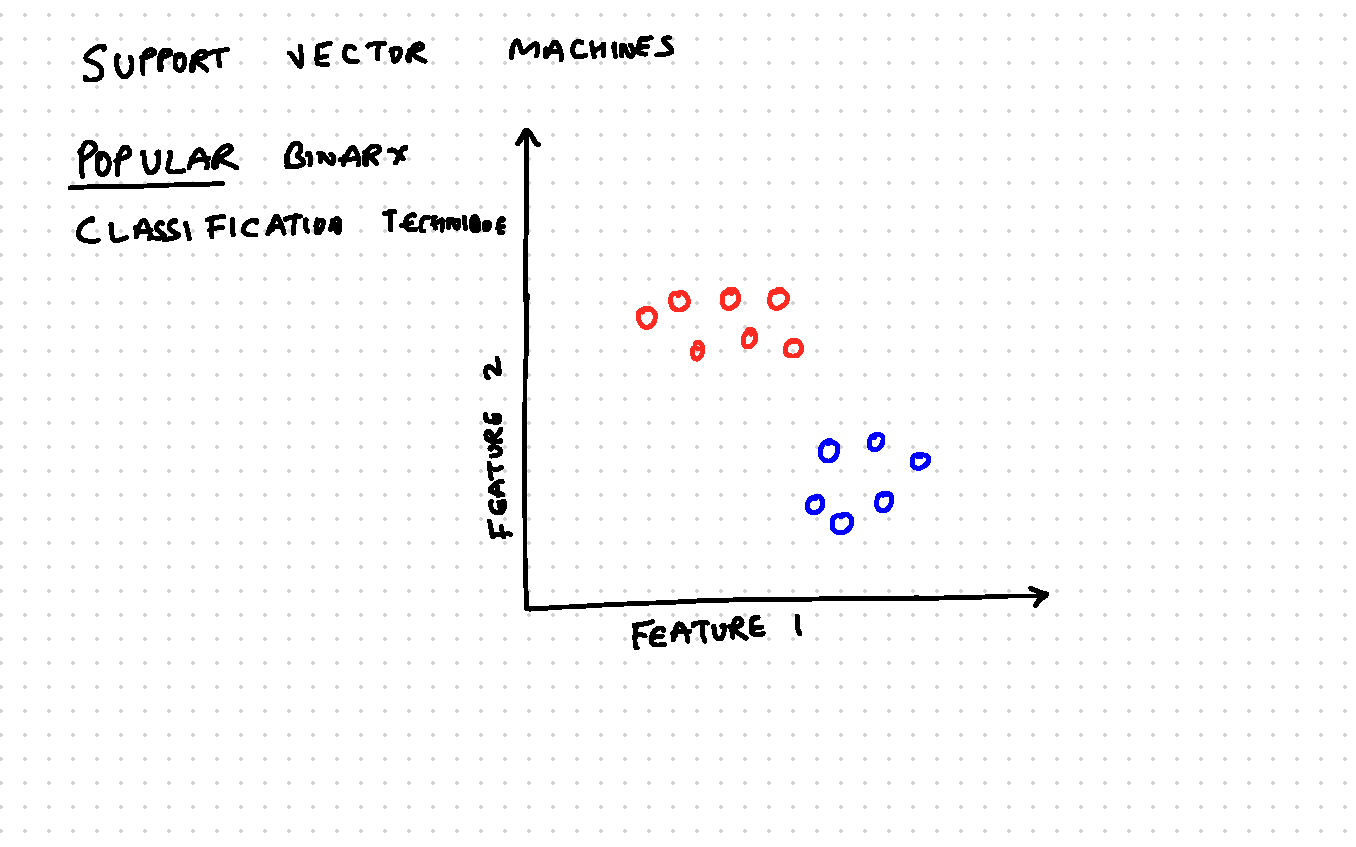
\includepdf[page=28-33]{svm/Svm-notes.pdf}
}


\begin{frame}{Simple Exercise}

\begin{align*}
w_{min} = 1, b&= 0\\
w.x + b &= 0\\
x &=0 \\
\end{align*}

\end{frame}

\begin{frame}{Simple Exercise}
Minimum values satisfying constraints  $\Rightarrow$
$w$ = 1 and $b = 0$\\
$\therefore$ Max margin classifier $ \Rightarrow x = 0$

\end{frame}

\begin{frame}{Primal Formulation is a Quadratic Program}
\begin{align*}
\text{Generally;}&\\
&\Rightarrow \text{Minimize Quadratic(x)}\\
&\Rightarrow \text{such that, Linear(x)}
\end{align*}
\begin{tcolorbox}
Question
\begin{align*}
&{x} = (x_{1}, x_{2})\\
&\text{minimize} \hspace{3mm} \frac{1}{2}||x||^{2}\\
&\colon x_{1} + x_{2} - 1 \geq 0
\end{align*}
\end{tcolorbox}
\end{frame}



{
	\setbeamercolor{background canvas}{bg=}
	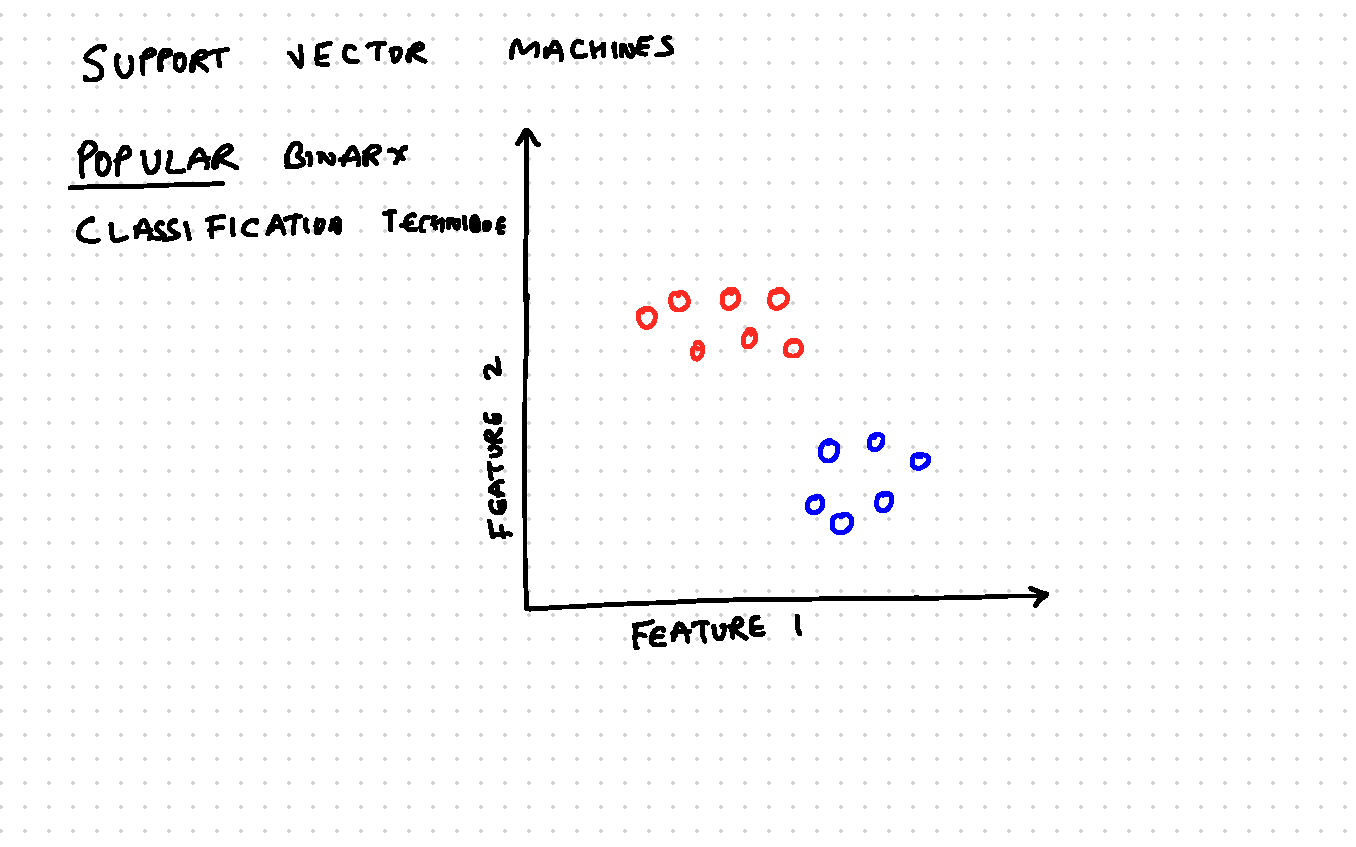
\includepdf[page=34]{svm/Svm-notes.pdf}
}



\begin{frame}{Converting to Dual Problem}
Primal $\Rightarrow$ Dual Conversion using Lagrangian multipliers\\
\begin{align*}
	\text{Minimize } & \frac{1}{2}||\bar{w}||^{2} \\
	\text{s.t. } & y_{i}(\bar{w}.x_{i} + b) \geq 1\\
	 \hspace{2mm}\forall i
	\end{align*}
\begin{align*}
&L(\bar{w},b,\alpha_{1},\alpha_{2},...\alpha_{n}) = \frac{1}{2}
\sum_{i = 1}^{d} w_{i}^{2} - \sum_{i=1}^{N} \alpha_{i}(y_{i}(\bar{w}.\bar{x_{i}} + b) - 1) \hspace{2mm} \forall \hspace{2mm}\alpha_{i} \geq 0\\
&\frac{\partial L}{\partial b} = 0 \Rightarrow \sum_{i=1}^{n}\alpha_{i}y_{i} = 0\\
\end{align*}
\end{frame}

\begin{frame}{Converting to Dual Problem}
\begin{align*}
\frac{\partial L}{\partial w} = 0 \Rightarrow & \bar{w} - \sum_{i=1}^{n}\alpha_{i}y_{i}\bar{x_{i}} = 0\\
& \bar{w} = \sum_{i=1}^{N}\alpha_{i}y_{i}\bar{x_{i}}
\end{align*}
\begin{align*}
&L(\bar{w},b,\alpha_{1},\alpha_{2},...\alpha_{n}) = \frac{1}{2}
\sum_{i = 1}^{d} w_{i}^{2} - \sum_{i=1}^{N} \alpha_{i}(y_{i}(\bar{w}.\bar{x_i} + b) -1\\
&= \frac{1}{2}||\bar{w}||^{2}-\sum_{i=1}^{N} \alpha_{i} y_{i} \vec{w}_{.} \bar{x_{i}}-\sum_{i=1}^{N} \alpha_{i} y_{i} b+\sum_{i=1}^{N} \alpha_{i}\\
&= \sum_{=1}^{N} \alpha_{i}+\frac{\left(\sum_{i} \alpha_{i} y_{i} \bar{x}_{i}\right)\left(\sum_{j} \alpha_{j} y_{j} \bar{x}_{j}\right)}{2}-\sum_{i} \alpha_{i} y_{i}\left(\sum_{j} \alpha_{j} y_{j} \bar{x}_{j}\right) \bar{x_{i}}
\end{align*}
\end{frame}

\begin{frame}{Converting to Dual Problem}
\begin{align*}
&L(\alpha)=\sum_{i=1}^{N} \alpha_{i}-\frac{1}{2} \sum_{i=1}^{N} \sum_{j=1}^{N} \alpha_{i} \alpha_{j} y_{i} y_{j} \bar{x_{i}} \cdot \bar{x_{j}}\\
\end{align*}
\begin{tcolorbox}
\begin{align*}
&\begin{array}{ll}
{\text { Minimize }\|\bar{w}\|^{2} \Rightarrow}&{\text{Maximize } L(\alpha)} \\
{  s.t  } & {  s.t  } \\
{y_{i}\left(\bar{w}, x_{i}+b\right) \geqslant 1} & {\sum_{i=1}^{N} \alpha_{i} y_{i}=0 \hspace{2mm}\forall \hspace{2mm} \alpha_{i}  \geq 0}
\end{array}
\end{align*}
\end{tcolorbox}
\end{frame}

\begin{frame}{Question}
\textbf{Question}:\\
\vspace{2mm}
$\alpha_{i}\left(y_{i}\left(\bar{w}, \bar{x}_{i}+b\right)-1\right)=0 \quad \forall i$ as per KKT slackness\\
\vspace{2mm}
What is $\alpha_{i}$ for support vector points?\\
\vspace{4mm}
\textbf{Answer:}
For support vectors,\\
\hspace{1in}$\bar{w}.\bar{x_{i}} + b  = -1$ (+ve class)\\
\hspace{1in}$\bar{w}.\bar{x_{i}} + b  = +1$ (+ve class)\\
\vspace{2mm}
$\left.y_{i}\left(\bar{w} \cdot \bar{x}_{i}+b\right)-1\right)=0 \quad \text {for } i=\{\text{support vector points\}}$
$\therefore \alpha_{i} \text { where i } \in \text{\{support vector points\}} \neq 0$
\vspace{5mm}
$\text{For all non-support vector points }\alpha_{i} = 0$
\end{frame}

{
	\setbeamercolor{background canvas}{bg=}
	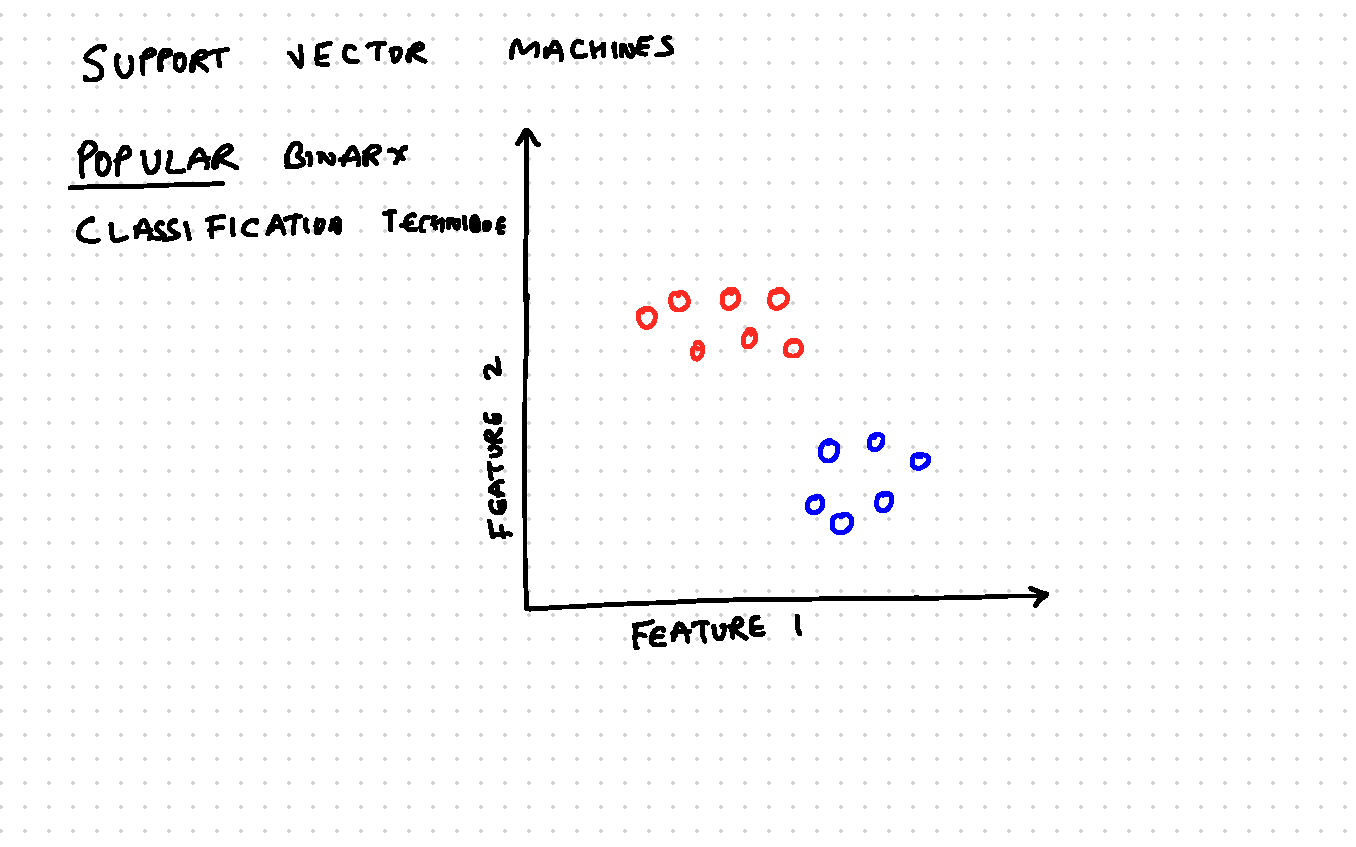
\includepdf[page=27]{svm/Svm-notes.pdf}
}


\begin{frame}{Revisiting the Simple Example}


\begin{equation*}
\begin{bmatrix}
x_{1} && y \\
1 && 1\\
2 && 1\\
-1 && -1\\
-2 && -1\\
\end{bmatrix}
\end{equation*}

\begin{align*}
L(\alpha) &= \sum_{i=1}^{4} \alpha_{i} - \frac{1}{2}\sum_{i=1}^{4}\sum_{j=1}^{4}\alpha_{i}\alpha_{j}y_{i}y_{j}\bar{x_i}\bar{x_j} \hspace{1cm}\alpha_{i} \geq 0 \\
&\sum \alpha_{i}y_{i} = 0 \hspace{1.5cm}
\alpha_{i}(y_{i}(\bar{w}.\bar{x_i} + b - 1) = 0
\end{align*}

\end{frame}

\begin{frame}{Revisiting the Simple Example}
\begin{align*}
\begin{aligned}
\left.L(\alpha_{1},\alpha_{2},\alpha_{3},\alpha_{4}\right)=& \alpha_{1}+\alpha_{2}+\alpha_{3}+\alpha_{4} \\
&-\frac{1}{2}\left\{\alpha_{1} \alpha_{1}\times(1*1) \times(1 * 1)\right.\\
&\hspace{1cm} + \\
& \alpha_{1} \alpha_{2} \times(1*1) \times(1*2) \\
&\hspace{1cm}+\\
& \alpha_{1} \alpha_{3} \times(1*-1)\times(1*1)\\
& \hspace{1cm} ... \\
& \alpha_4\alpha_4 \times(-1*-1)\times(-2*-2)
\}
\end{aligned}
\end{align*}
How to Solve? $\Rightarrow$ Use the QP Solver!!
\end{frame}

\begin{frame}{Revisiting the Simple Example}
For the trivial example, \\
We know that only x = $\pm 1$ will take part in the constraint actively. Thus, $\alpha_2, \alpha_{4} = 0$ \\
\hspace{2cm} By symmetry, $\alpha_{1} = \alpha_{3} = \alpha $\text{ (say) }\\
\hspace{2cm} \& $\sum y_i\alpha_i = 0$
\begin{align*}
\begin{aligned}
\left.L(\alpha_{1},\alpha_{2},\alpha_{3},\alpha_{4}\right)=& 2\alpha \\
&-\frac{1}{2}\left\{\alpha^{2} (1)(-1)(1)(-1) \right. \\
&\hspace{1cm} + \alpha^{2} (-1)(1)(-1)(1) \\
&\hspace{1cm} + \alpha^{2} (1)(1)(1)(1) +  \alpha^{2} (-1)(-1)(-1)(-1) \\
\}\\
\end{aligned}
\end{align*}
\hspace{2cm} $\underset{\alpha}{Maximize} \hspace{3mm} 2\alpha - \frac{1}{2}(4\alpha^{2})$
\end{frame}

\begin{frame}{Revisiting the Simple Example}
\begin{align*}
\begin{aligned}
\frac{\partial}{\partial \alpha}\left(2 \alpha- 2\alpha^{2}\right)=0 & \Rightarrow 2-4 \alpha=0 \\
\Rightarrow \hspace{2mm}& \alpha=1/2\\
\end{aligned}\\
\therefore \alpha_{1}=1/2 \hspace{2mm} \alpha_{2}=0 ; \hspace{2mm} \alpha_{3}=1/2 \hspace{2mm} \alpha_{4}=0
\\
\vec{w}=\sum_{i=1}^{N} \alpha_{i} y_{i} \bar{x}_{i} =1/2 \times 1 \times 1+0 \times 1 \times 2 \\
+ 1/2 \times -1 \times -1 + 0\times -1 \times -2 \\
 = 1/2 + 1/2 = 1
\end{align*}
\end{frame}

\begin{frame}{Revisiting the Simple Example}
\textbf{Finding b:}\\
For the support vectors we have, \\

$y_{i}(\vec{w} \cdot \overrightarrow{x_{i}}+b)-1=0$\\
or, $y_{i}$ $\left(\bar{w} \cdot \bar{x}_{1}+b\right)=1$\\
or, $y_{i}^{2}\left(\bar{w} \cdot \bar{x}_{i}+b\right)=y_{i}$\\
or, $\quad \bar{w}, \bar{x}_{i}+b=y_{i} \hspace{2mm}(\because y_{i}^{2} = 1)$\\
or, $b= y_i - w \cdot x_i$

In practice, $b=\frac{1}{N_{SV}} \sum_{i=1}^{N_{SV}}\left(y_{i}-\bar{w}\bar{x}_{i}\right)$

\end{frame}

\begin{frame}{Obtaining the Solution}
\begin{align*}
\begin{aligned}
b &=\frac{1}{2}\{(1-(1)(1))+(-1-(1)(-1))\\
&=\frac{1}{2}\{0+0\}=0 \\
&=0 \\
& \therefore w = 1 \hspace{2mm}\& \hspace{2mm} b = 0
\end{aligned}
\end{align*}
\end{frame}

\begin{frame}{Making Predictions}
\textbf{Making Predictions} \\
\hspace{2cm} $\hat{y}(x_i) = \operatorname{SIGN}(w \cdot x_i + b)$\\

For $x_{test} = 3$; $\hat{y}(3) = \operatorname{SIGN}(1 \times 3 + 0)$ = +ve class
\end{frame}

\begin{frame}{Making Predictions}\
\begin{align*}
\begin{array}{l}
{\text {Alternatively, }} \\
{\qquad \begin{aligned}
\hat{y}\left(x_{TEST}\right) &=\operatorname{SIGN}\left(\bar{w} \cdot \bar{x}_{TEST}+b\right) \\
&=\operatorname{SIGN} \left(\sum_{i=1}^{N_{S}} \alpha_{j} y_{j} x_{j} \cdot x_{test}+b\right)
\end{aligned}}
\end{array}
\end{align*}
\begin{align*}
\begin{aligned}
&\text{In our example,} \\
&\alpha_{1}=1/2 ; \alpha_{2}=0 ; \quad \alpha_{3}=1/2 ; \alpha_{4}=0\\
&\hat{y}(3) =\operatorname{SIGN}\left(\frac{1}{2} \times 1 \times (1 \times 3)+0+\frac{1}{2} \times (-1) \times (-1 \times 3)+0\right)\\
&=\operatorname{SIGN} \left(\frac{6}{2}\right)=\operatorname{SIGN}(3)=+1
\end{aligned}
\end{align*}

\end{frame}


\end{document}